% -*- LaTeX -*-
% -*- coding: utf-8 -*-
%
% michael a.g. aïvázis <michael.aivazis@para-sim.com>
% (c) 2003-2017 all rights reserved
%

\section{introduction}

%-----------------------------------
\begin{frame}[c,plain]
  \begin{center}
    
\includegraphics[width=0.75\textwidth]{pyre-logo}
  \end{center}
\end{frame}


% -----------------------------------
\begin{frame}
%
  \frametitle{Introduction}
%
  \vskip -3ex
  \begin{itemize}
%
  \item \pyre\ is a strategy for
    \begin{itemize}
    \item managing code complexity
    \item integrating third party tools and libraries into a coherent whole
    \item empowering the end-user to make critical decisions about the composition of an
      application while minimizing the risk of compromising its integrity
    \end{itemize}
%
    \item \pyre\ extends object oriented ideas
      \begin{itemize}
      \item abstract base classes become \emph{protocols}
      \item appropriately decorated classes become \emph{components}
      \item design and implement by contract
      \end{itemize}
%
    \item \pyre\ is also a powerful computational environment with rich services
      \begin{itemize}
      \item application configuration
      \item launching and staging in serial, parallel, distributed modes
      \item logging and monitoring
      \item special services for interacting with users via the production of structured
        documents
        \begin{itemize}
        \item think \html\ for web applications, remote UIs
        \end{itemize}
      \item name and filesystem abstractions
      \item powerful lazy evaluation mechanisms
      \item seamless access to database back-ends without the need for direct access using
        embedded \sql\ or similar techniques
      \end{itemize}
%
  \end{itemize}
%
\end{frame}

% -----------------------------------
\begin{frame}
%
  \frametitle{Outline}
%
  \begin{itemize}
%
  \item \isce\ 3.0 hides \pyre\ completely from its users
    \begin{itemize}
    \item so even though this is about the framework, the word \pyre\ won't show up much
    \end{itemize}
%
  \item we will write an \isce\ application that stitches together a digital elevation model
    (\dem) by downloading tiles from the \srtm\ archive
%
  \item we will separate \emph{mechanism} from \emph{interface} by writing
    \begin{itemize}
    \item a class that knows how to interact with the \srtm\ archive
    \item a harness that enables the user to orchestrate the interaction
    \end{itemize}
%
  \item our goal is to
    \begin{itemize}
    \item become familiar with components, and their properties and behaviors
    \item describe the configuration process from the end user's point of view
    \item build a simple pyre application that instantiates and exercises a component
    \item gradually transform the app into a capability that is integrated into an open ended
      environment
    \end{itemize}
%
  \item much of the code in these examples is lifted straight out of the \isce\ 3.0 source
    code.
%
  \item as we go along, we will introduce notation that makes it possible to discuss
    application architecture without the complexity of having to show actual source code. The
    notation is inspired by \uml\supercite{uml-99,uml-05}, but is significantly simpler.
%
  \end{itemize}
%
\end{frame}

% -----------------------------------
\begin{frame}[t]
  \frametitle{Stitching together a digital elevation model}
%
  \vskip -3ex
%
  The basic idea is very simple:
%
    \begin{columns}
      \begin{column}{.4\textwidth}
        \only<1>{
          \begin{center}
            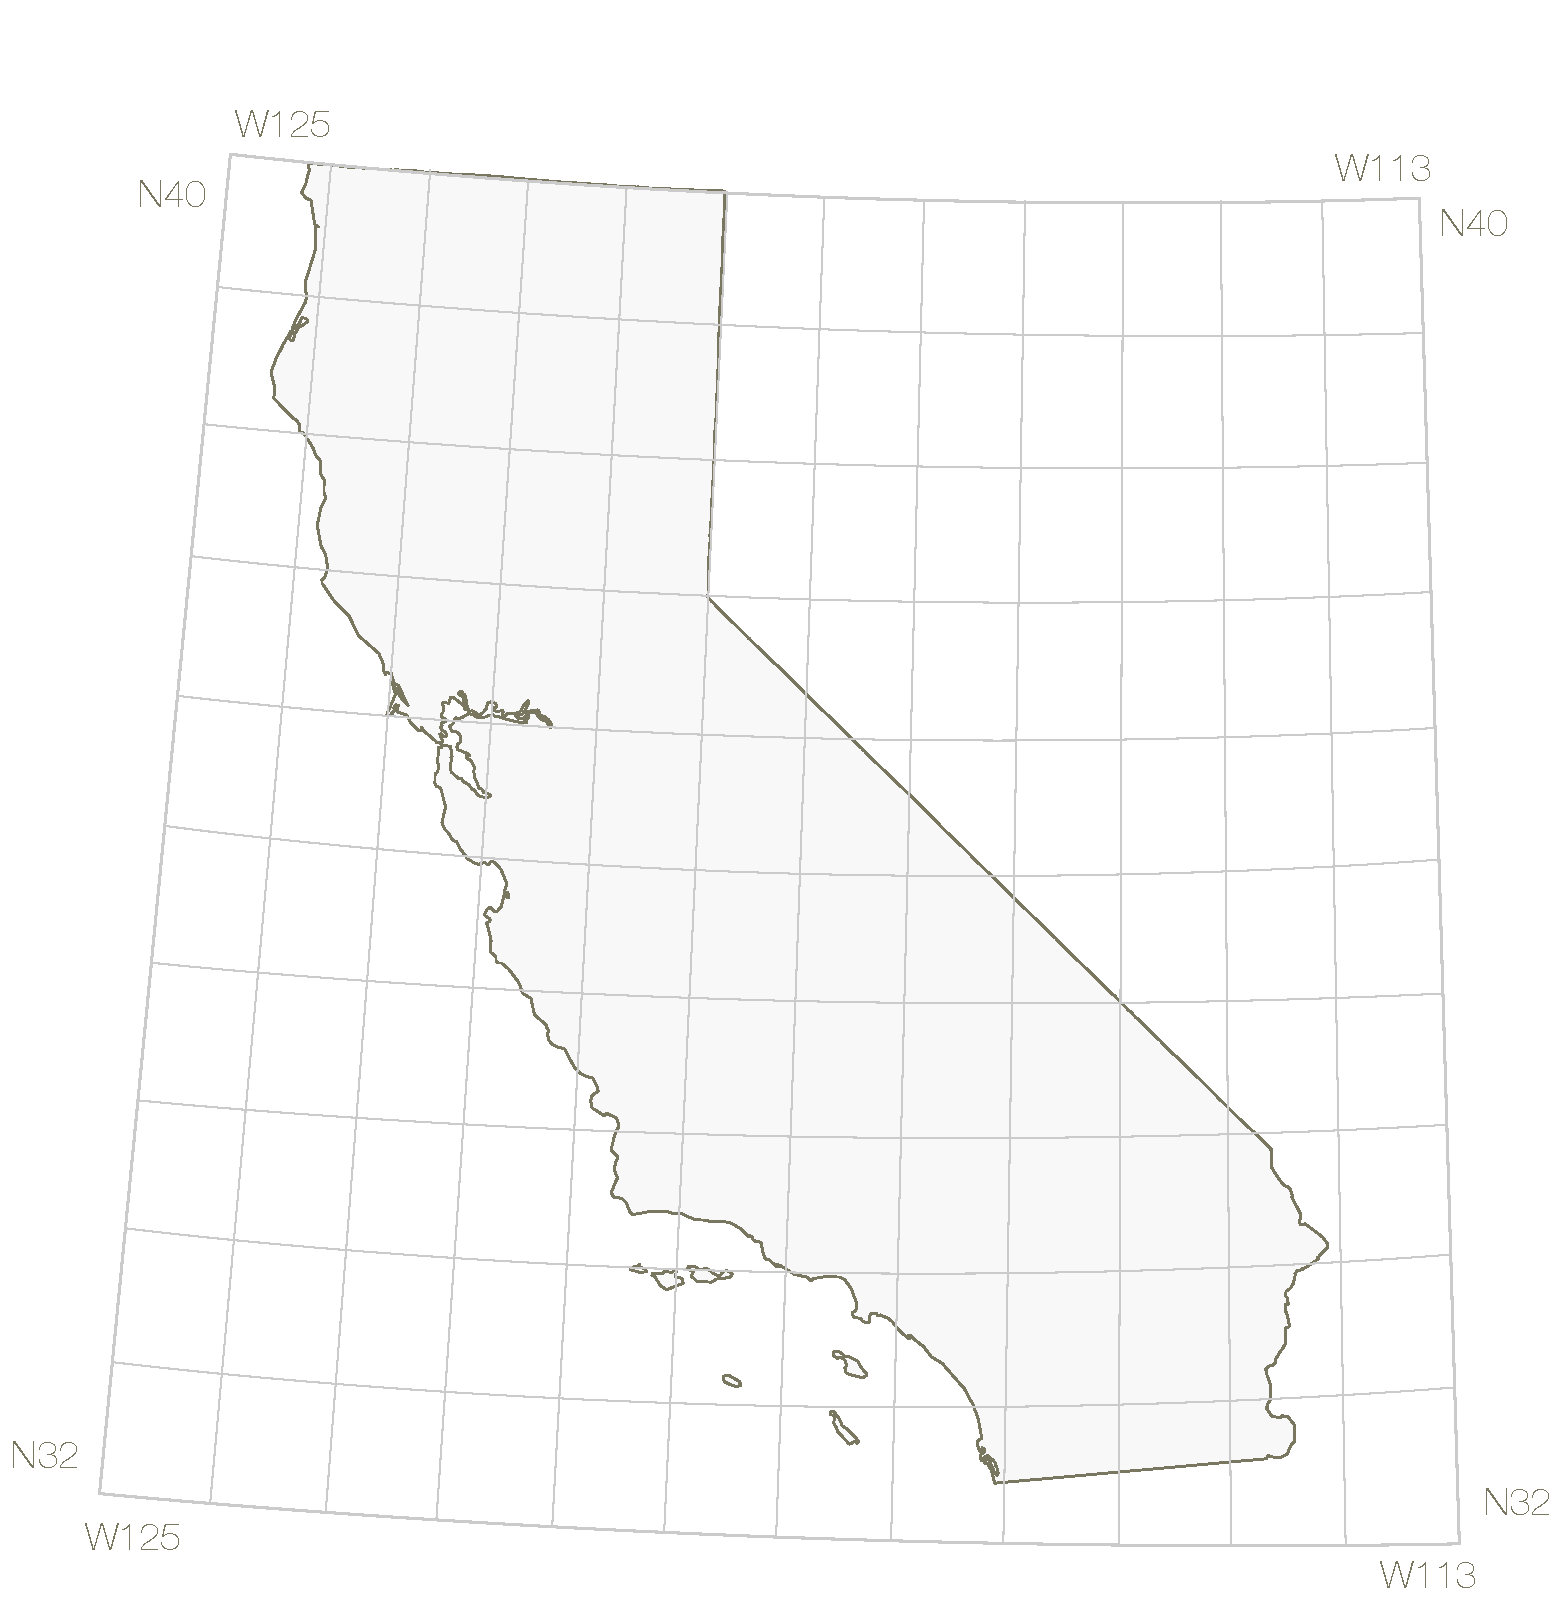
\includegraphics[width=\textwidth]{dem-california}
          \end{center}
        }
        \only<2>{
          \begin{center}
            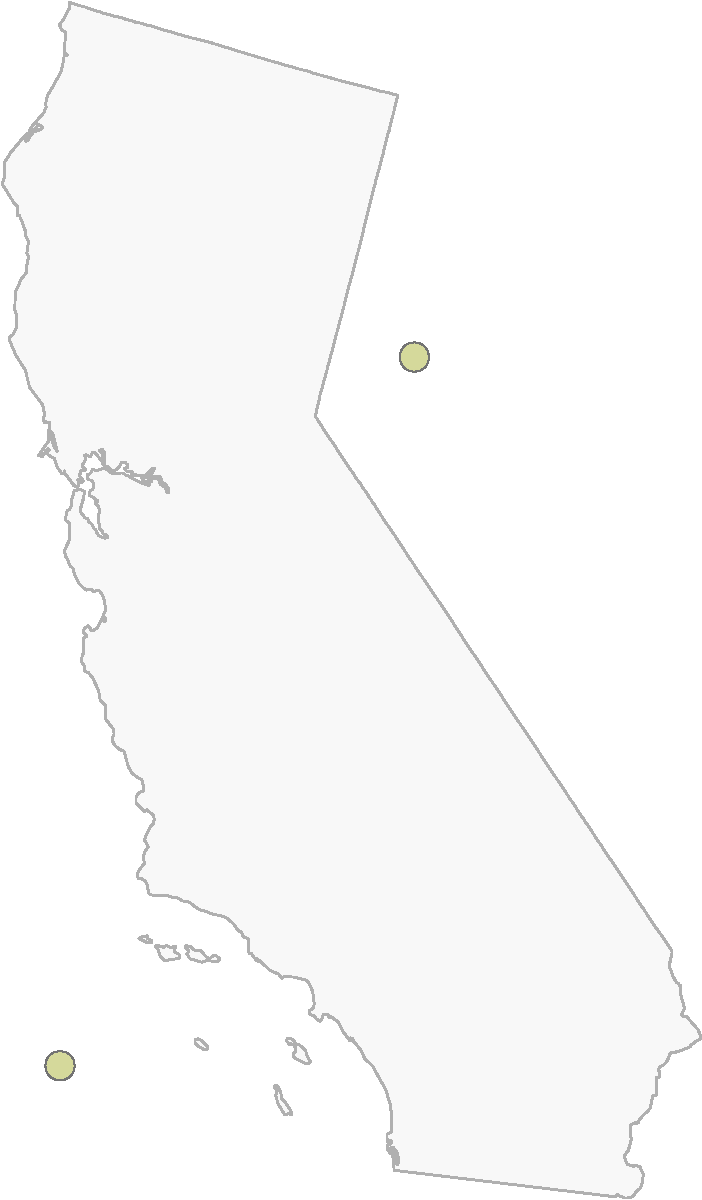
\includegraphics[width=\textwidth]{dem-region}
          \end{center}
        }
        \only<3>{
          \begin{center}
            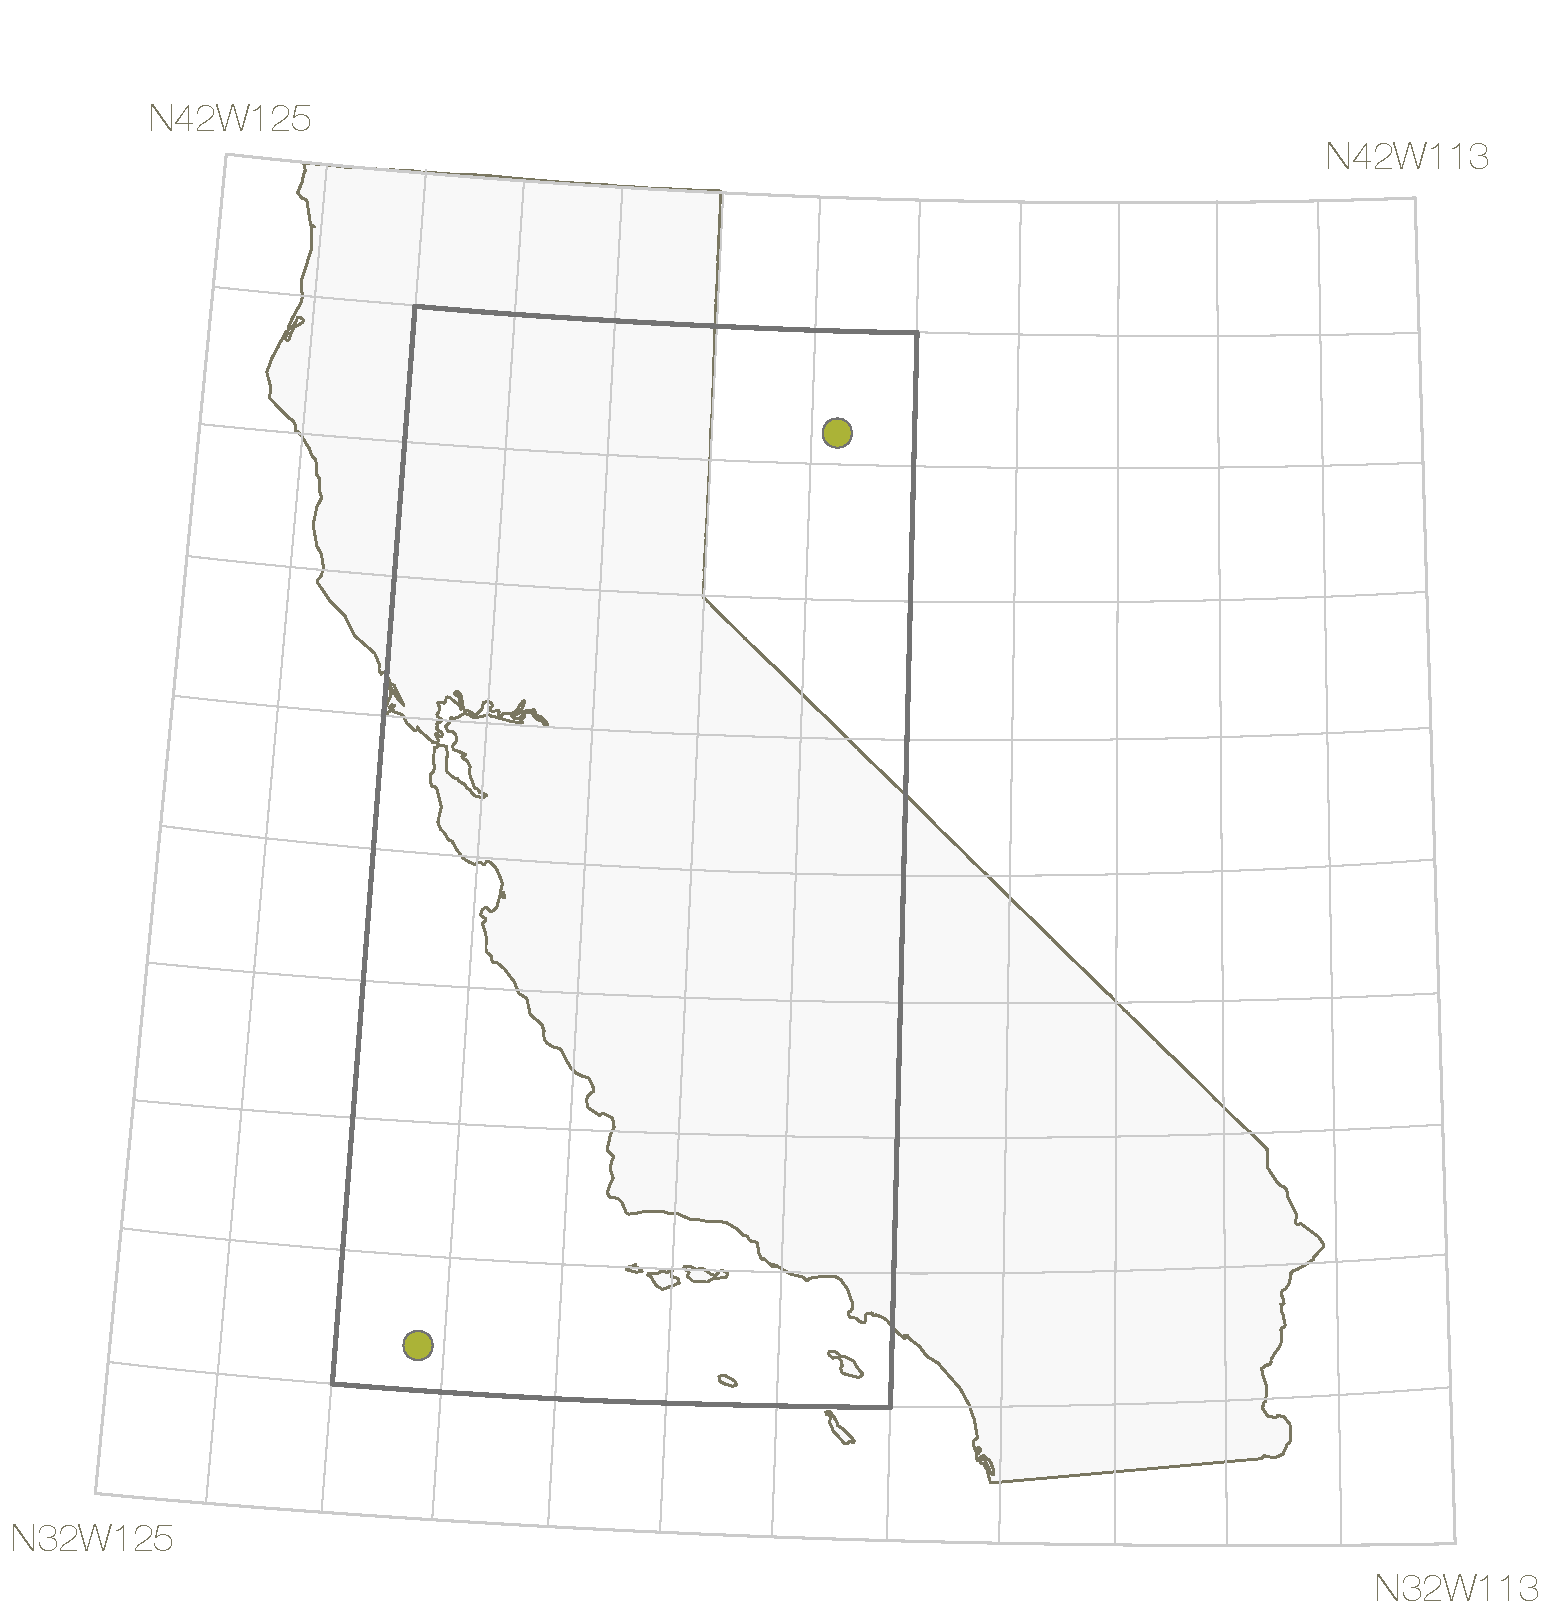
\includegraphics[width=\textwidth]{dem-bbox}
          \end{center}
        }
        \only<4->{
          \begin{center}
            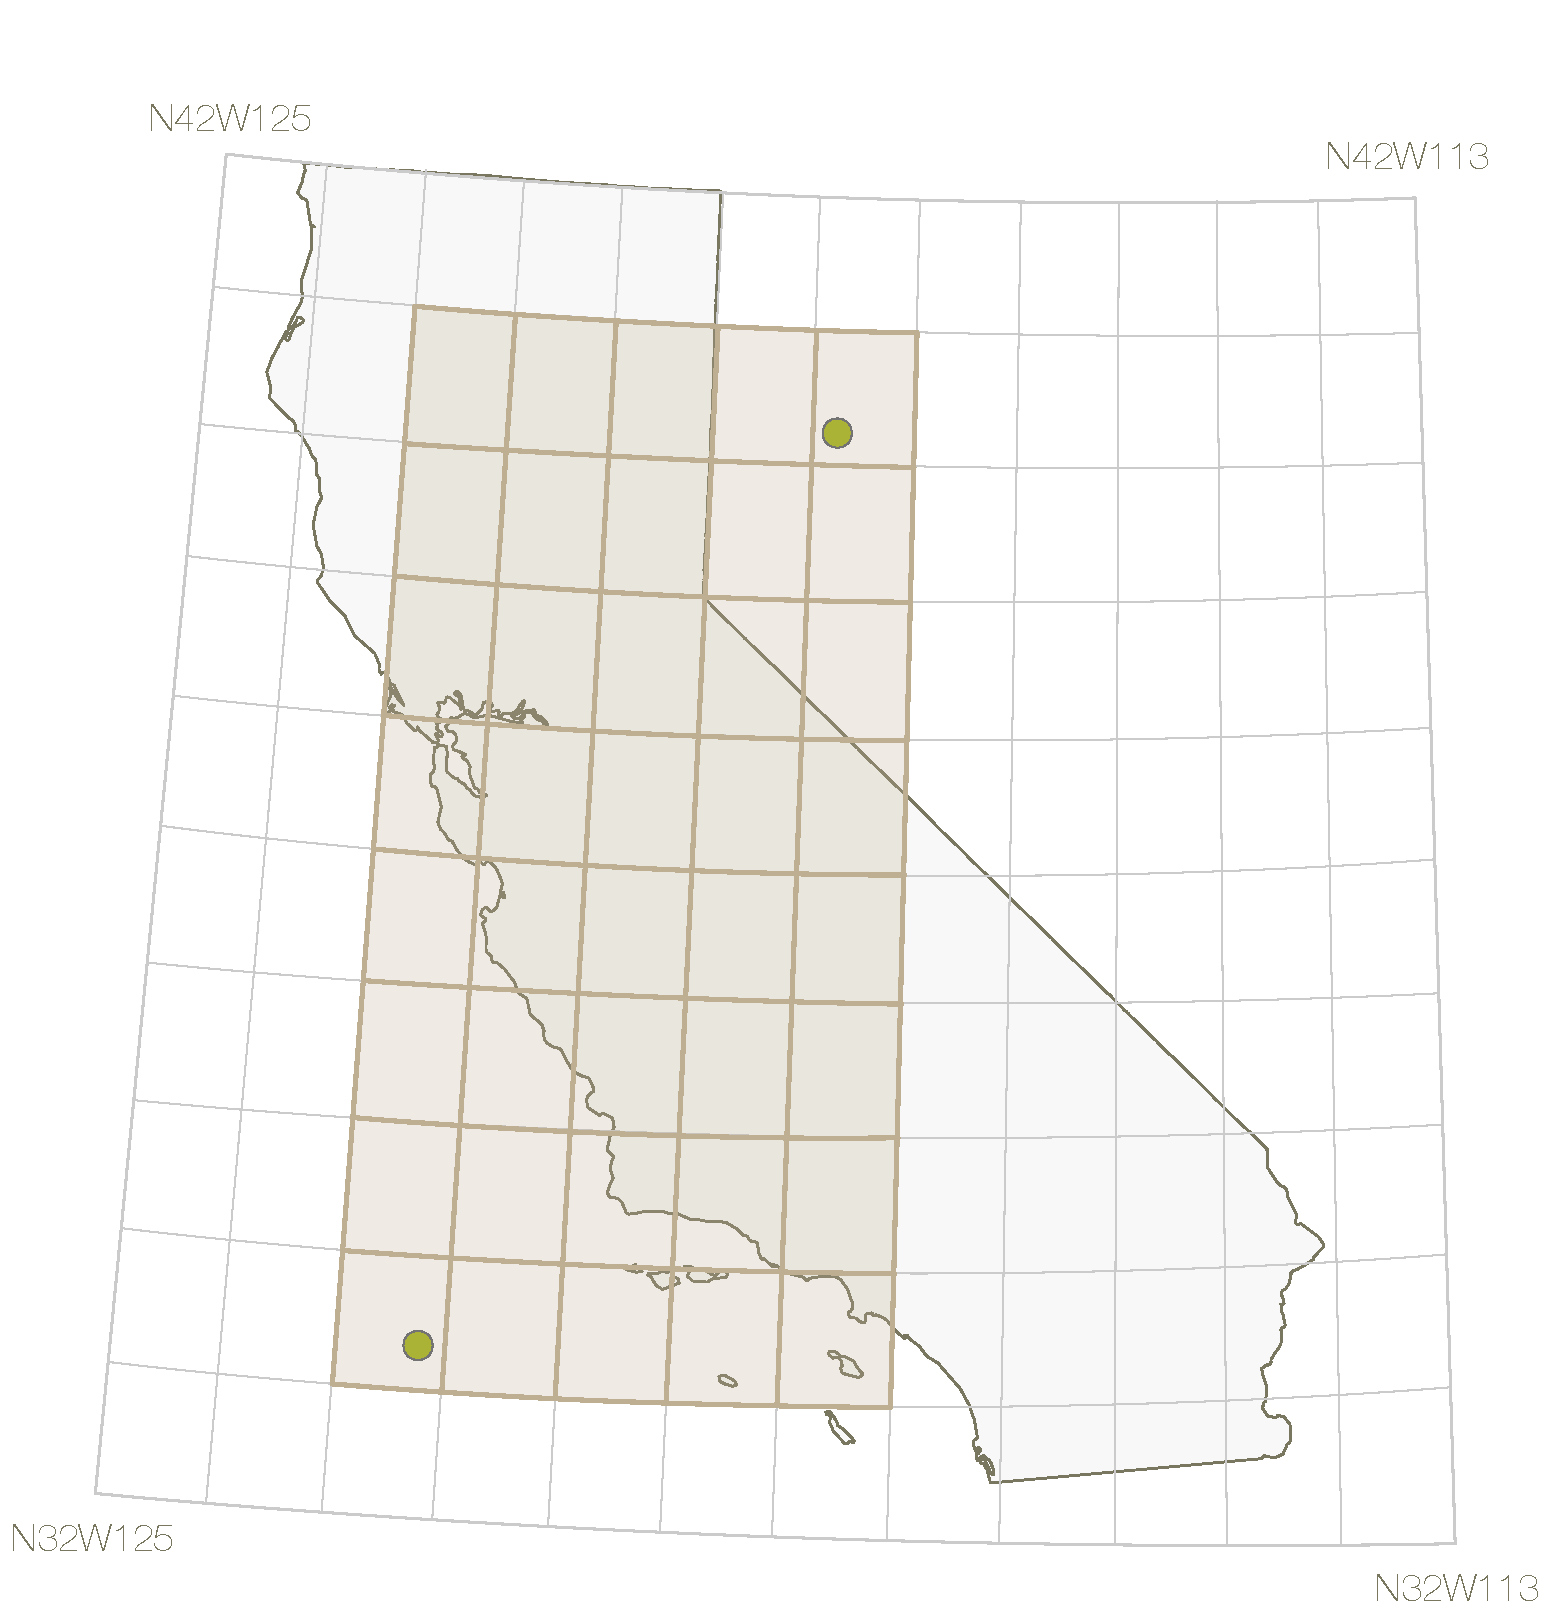
\includegraphics[width=\textwidth]{dem-tiles}
          \end{center}
        }
      \end{column}
%
      \begin{column}{.6\textwidth}
        \begin{itemize}
        \item<2-> the user picks a few points in a region of interest
        \item<3-> we compute an axis-aligned bounding box
        \item<4-> fill the box with $1\si{\degree} \times 1\si{\degree}$ tiles
        \item<5-> download the \dem\ tiles from the \srtm\ data store
        \item<6-> stitch the \dem\ together and drop it somewhere on the filesystem
        \end{itemize}
      \end{column}
%
    \end{columns}

    \only<7->{ \vskip 2ex Transforming the idea into an actual running program will require
      more information, and many decisions.  A key aspect of the design process is to identify
      which decisions are best left to the end user, and therefore become configuration options
      for our app.}
%
\end{frame}

%%% Local Variables:
%%% mode: latex
%%% TeX-master: "../pyre"
%%% End:

% end of file
